% 这是中国科学院大学计算机科学与技术专业《计算机组成原理（研讨课）》使用的实验报告 Latex 模板
% 本模板与 2024 年 2 月 Jun-xiong Ji 完成, 更改自由 Shing-Ho Lin 和 Jun-Xiong Ji 于 2022 年 9 月共同完成的基础物理实验模板
% 如有任何问题, 请联系: jijunxoing21@mails.ucas.ac.cn
% This is the LaTeX template for report of Experiment of Computer Organization and Design courses, based on its provided Word template. 
% This template is completed on Febrary 2024, based on the joint collabration of Shing-Ho Lin and Junxiong Ji in September 2022. 
% Adding numerous pictures and equations leads to unsatisfying experience in Word. Therefore LaTeX is better. 
% Feel free to contact me via: jijunxoing21@mails.ucas.ac.cn

\documentclass[11pt]{article}

\usepackage[a4paper]{geometry}
\geometry{left=2.0cm,right=2.0cm,top=2.5cm,bottom=2.5cm}

\usepackage{ctex} % 支持中文的LaTeX宏包
\usepackage{amsmath,amsfonts,graphicx,subfigure,amssymb,bm,amsthm,mathrsfs,mathtools,breqn} % 数学公式和符号的宏包集合
\usepackage{algorithm,algorithmicx} % 算法和伪代码
\usepackage[noend]{algpseudocode} % 算法和伪代码
\usepackage{fancyhdr} % 自定义页眉页脚
\usepackage[framemethod=TikZ]{mdframed} % 创建带边框的框架
\usepackage{fontspec} % 字体设置
\usepackage{adjustbox} % 调整盒子大小
\usepackage{fontsize} % 设置字体大小
\usepackage{tikz,xcolor} % 绘制图形和使用颜色
\usepackage{multicol} % 多栏排版
\usepackage{multirow} % 表格中合并单元格
\usepackage{pdfpages} % 插入PDF文件
\usepackage{listings} % 在文档中插入源代码
\usepackage{wrapfig} % 文字绕排图片
\usepackage{bigstrut,multirow,rotating} % 支持在表格中使用特殊命令
\usepackage{booktabs} % 创建美观的表格
\usepackage{circuitikz} % 绘制电路图
\usepackage{zhnumber} % 中文序号（用于标题）
\usepackage{tabularx} % 表格折行
\usepackage{dirtree}
\usepackage{verbatimbox}

\definecolor{CPPLight}  {HTML} {686868}
\definecolor{CPPSteel}  {HTML} {888888}
\definecolor{CPPDark}   {HTML} {262626}
\definecolor{CPPBlue}   {HTML} {4172A3}
\definecolor{CPPGreen}  {HTML} {487818}
\definecolor{CPPBrown}  {HTML} {A07040}
\definecolor{CPPRed}    {HTML} {AD4D3A}
\definecolor{CPPViolet} {HTML} {7040A0}
\definecolor{CPPGray}  {HTML} {B8B8B8}
\lstset{
    columns=fixed,       
    % numbers=left,                                        % 在左侧显示行号
    frame=none,                                          % 不显示背景边框
    backgroundcolor=\color[RGB]{245,245,244},            % 设定背景颜色
    keywordstyle=\color[RGB]{40,40,255},                 % 设定关键字颜色
    numberstyle=\footnotesize\color{darkgray},           % 设定行号格式
    commentstyle=\it\color[RGB]{0,96,96},                % 设置代码注释的格式
    stringstyle=\rmfamily\slshape\color[RGB]{128,0,0},   % 设置字符串格式
    showstringspaces=false,                              % 不显示字符串中的空格
    language=verilog,                                        % 设置语言
    morekeywords={default,reg,wire,assign,module,endmodule,always,input,output,alignas,continute,friend,register,true,alignof,decltype,goto,
    reinterpret_cast,try,asm,defult,if,return,typedef,auto,delete,inline,short,
    typeid,bool,do,int,signed,typename,break,double,long,sizeof,union,case,
    dynamic_cast,mutable,static,unsigned,catch,else,namespace,static_assert,using,
    char,enum,new,static_cast,virtual,char16_t,char32_t,explict,noexcept,struct,
    void,export,nullptr,switch,volatile,class,extern,operator,template,wchar_t,
    const,false,private,this,while,constexpr,float,protected,thread_local,xnor,
    const_cast,for,public,throw,std},
    emph={map,set,multimap,multiset,unordered_map,unordered_set,
    unordered_multiset,unordered_multimap,vector,string,list,deque,
    array,stack,forwared_list,iostream,memory,shared_ptr,unique_ptr,
    random,bitset,ostream,istream,cout,cin,endl,move,default_random_engine,
    uniform_int_distribution,iterator,algorithm,functional,bing,numeric,begin,end},
    emphstyle=\color{CPPViolet}, 
}

\definecolor{dkgreen}{rgb}{0,0.6,0}
\definecolor{gray}{rgb}{0.5,0.5,0.5}
\definecolor{mauve}{rgb}{0.58,0,0.82}
\lstset{
  frame=tb,
%   numbers=left,
  aboveskip=3mm,
  belowskip=3mm,
  showstringspaces=false,
  columns=flexible,
  framerule=1pt,
  rulecolor=\color{gray!35},
  backgroundcolor=\color{gray!5},
  basicstyle={\small\ttfamily},
  numberstyle=\tiny\color{gray},
  keywordstyle=\color{blue},
  commentstyle=\color{dkgreen},
  stringstyle=\color{mauve},
  breaklines=true,
  breakatwhitespace=true,
  tabsize=3,
}

% 轻松引用, 可以用\cref{}指令直接引用, 自动加前缀. 
% 例: 图片label为fig:1
% \cref{fig:1} => Figure.1
% \ref{fig:1}  => 1
\usepackage[capitalize]{cleveref}
% \crefname{section}{Sec.}{Secs.}
\Crefname{section}{Section}{Sections}
\Crefname{table}{Table}{Tables}
\crefname{table}{Table.}{Tabs.}

% \setmainfont{Palatino Linotype.ttf}
% \setCJKmainfont{SimHei.ttf}
% \setCJKsansfont{Songti.ttf}
% \setCJKmonofont{SimSun.ttf}
\punctstyle{kaiming}
% 偏好的几个字体, 可以根据需要自行加入字体ttf文件并调用

\renewcommand{\emph}[1]{\begin{kaishu}#1\end{kaishu}}

% 对 section 等环境的序号使用中文，按 1 / 1.1 / 1.1.1 的层级显示
\setcounter{secnumdepth}{3} % 显示到 subsubsection
\renewcommand\thesection{\arabic{section}}
\renewcommand\thesubsection{\thesection.\arabic{subsection}}
\renewcommand\thesubsubsection{\thesubsection.\arabic{subsubsection}}


%%%%%%%%%%%%%%%%%%%%%%%%%%%
%改这里可以修改实验报告表头的信息
\newcommand{\name}{薛翼舟}
\newcommand{\major}{计算机科学与技术}
%%%%%%%%%%%%%%%%%%%%%%%%%%%

\begin{document}

\begin{center}
  \LARGE \bf 中国科学院大学 \\《自然语言处理》实验报告
\end{center}

\begin{center}
  \emph{姓名} \underline{\makebox[8em][c]{\name}} 
  % 如果名字比较长, 可以修改box的长度"8em"为其他值
  \emph{专业} \underline{\makebox[15em][c]{\major}}\\
\end{center}


  

\section{实验题目}
\begin{figure}[H]
    \centering
    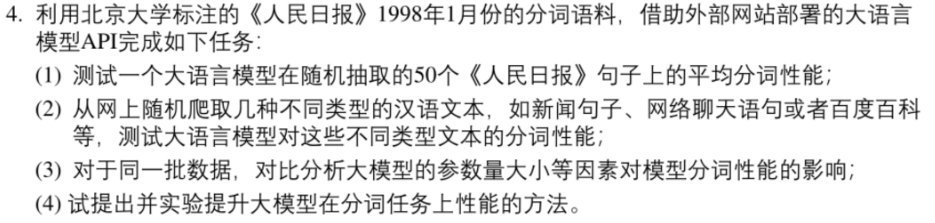
\includegraphics[width=0.9\textwidth]{fig/problem.png}
    \caption{实验题目}
\end{figure}

\section{设计讲解}
在本次实验中，我的实验代码目录如下，在这里不多赘述每部分代码的具体
功能，只对关键部分和实验结果进行讲解
\newline

\begin{lstlisting}
nlp作业3/
├── input/
│   └── ChineseCorpus199801.txt   # 原训练语料（你已经放进来了）
├── data/
│   └── sampled_50.json           # 执行脚步后自动提取的50句测试集（包含原始句和切分标准答案）
        comparison_result_deepseek-chat # deepseek-v4-flash的快速模式
        comparison_result_deepseek-reasoner # deepseek-v4-flash的思考模式
├── scripts/
│   ├── data_process.py           # 预处理与抽样脚本
│   ├── evaluate.py               # Precision, Recall, F1 计算指标脚本
│   └── task1_llm_pku.py          # 调用大模型执行任务1的核心脚本
└── README.md
\end{lstlisting}

\subsection{代码设计讲解}
\subsubsection{data_process.py}
这个脚本的作用是将原始物料中的词性等消去，得到纯文本的语料，并从中随机抽取50句作为测试集，保存在data目录下的sampled\_50.json中。每条数据包含原始句和切分标准答案两部分。
\subsubsection{task1_llm_pku.py}
这个脚本主要是将data目录下的sampled\_50.json中的每条数据输入到这个脚本中所调用的大模型对话中，
在这个脚本中，首先要根据对应的模型的要求调用好apikey和url接口，然后设计好prompt，最后将每条数据输入到大模型中，
得到切分结果，并将结果保存在data目录下的comparison\_result\_deepseek-chat.json和comparison\_result\_deepseek-reasoner.json中，分别对应deepseek-v4-flash的快速模式和思考模式。
\subsection{evaluate.py}
在本次实验中，主要有以下三个评估指标
\begin{itemize}
    \item Precision: 预测正确的词语数量占预测结果中词语总数量的比例
    \item Recall: 预测正确的词语数量占标准答案中词语总数量的比例
    \item F1 Score: Precision和Recall的调和平均数，综合考虑了Precision和Recall的表现
\end{itemize}
并将结果保存在data目录下的comparison\_result\_deepseek-chat.json
和comparison\_result\_deepseek-reasoner.json中，分别对应deepseek-v4-flash的快速模式和思考模式。

\section{结果分析}
\subsection{人民日报1998年1月份语料分析结果}
根据输出文件的结果，快速模式的评估结果如下
\begin{lstlisting}
      "overall_metrics": 
        "precision": 0.8747,
        "recall": 0.8303,
        "f1_score": 0.8507
\end{lstlisting}
思考模式的评估结果如下
\begin{lstlisting}
      "overall_metrics": 
        "precision": 0.8429,
        "recall": 0.771,
        "f1_score": 0.8018
\end{lstlisting}
我们发现，相比之下，上下文更少，思考深度更浅的chat反而效果更好，但是经过检查二者最后输出的json文件发现，二者的差异主要体现在以下几个方面
\begin{itemize}
    \item 对于专有名词和任命的切分，比如在遇到日本人名如“早川泰伸殿”时，标准答案是合并的（早川泰伸殿），Reasoner 预测为合并（早川泰伸殿），符合标准答案；而 Chat 预测则倾向于将其切碎（早川 泰伸 殿）
    另外值得一提的是在遇到中文名词，比如“钱其琛”的时候， 标准答案会将姓和名拆开成“钱”，“其琛”。但是Chat和Reasoner都倾向于将其合并成“钱其琛”。这也导致了二者的分数都不是很高
    \item 对数词和量词的切分，chat和标准答案都倾向于拆开
    \item 对于一些复合词和专业术语如“催花量”，标准答案为 催花 量。这里 Chat 将其拆分开（催花 量），而 Reasoner 预测则倾向合并成一体（催花量）
\end{itemize}
综上所述，经过我仔细观察了分词的输出，chat和reasoner都没有明显的错误，所以这里的分数指的是他们的分词偏好和北京大学这个分词物料的相似程度，
事实上并不能完全代表他们的分词预测准确性。而之所以Chat的分数更高，可能因为它在一些常见词法规则和普通语句的细粒度切分上，更加契合现有的该
评测数据集（PKU 语料库等）的标准；而 DeepSeek-Reasoner 更倾向于“偏粗”的词语切分（比如更容易把人名、名词短语作为一个整体长词输出）。
\subsection{提升大模型分词任务性能的方法}
通过上个任务可以看出，为了得到不同的语料的不同分词结果，我们最直接的办法就是在prompt上做文章，比如说我给几个例子，让他更贴近我们标准答案的分词结果。
例如我把原本的prompt
\begin{lstlisting}
你是一流的中文语言学专家。请对下面的句子进行中文分词，词与词之间请用空格隔开，保留所有标点符号。
不要输出任何解释性的废话，只输出分词后的纯文本结果。
\end{lstlisting}
修改成
\begin{lstlisting}
你是一流的中文语言学专家。请对下面的句子按照以下示例进行中文分词，要注意中国人名的姓和名分开，
例如“钱其琛”解析成“钱 其琛”，还有复合词也要切分，另外数次和两次也分开，例如“1月份”切分成
“1 月份”。词与词之间请用空格隔开，保留所有标点符号。不要输出任何解释性的废话，
每个分词后也不要有斜杠和词性，只输出分词后的纯文本结果。
\end{lstlisting}
DeepSeed-Chat的结果提升到了
\begin{lstlisting}
    "overall_metrics": 
        "precision": 0.8539
        "recall": 0.8553
        "f1_score": 0.8526
\end{lstlisting}
另外，为了也可以将标准答案作为语料喂给大模型进行学习，来达到我们想要的分词效果.
\subsection{对百度百科的分词效果}
在这一部分中，我采用了https://github.com/guhhhhaa/4675-scifi中的科幻小说《流浪地球》和
https://huggingface.co/datasets/0xDing/wikipedia-cn-20230720-filtered/中的维基百科进行分词测试，
我原本来向也将百度贴吧中的对话作为语料输入，但是噪声实在是太大，遂放弃\par

在这个实验中，我用jieba作为标准答案，最终得到的结果如下, 科幻小说的分词结果如下
\begin{lstlisting}
        "metrics": 
            "precision": 0.8693,
            "recall": 0.8537,
            "f1_score": 0.8606
\end{lstlisting}
维基百科的分词结果如下
\begin{lstlisting}
        "metrics": 
            "precision": 0.7093,
            "recall": 0.6867,
            "f1_score": 0.6926
\end{lstlisting}
我们可以看到，chat的分词结果在科幻小说中更和jieba相似。但是我观察分词的比对结果发现，和上一个任务相同，
依然有很多“假错误”，例如科幻小说中的
\begin{lstlisting}
    "原句": "“重元素聚变是一门很深的学问，现在给你们还讲不明白。",
    "参考标准答案(Jieba)": "“ 重元素 聚变 是 一门 很深 的 学问 ， 现在 给 你们 还 讲 不 明白 。",
    "deepseek-chat预测": "重元素 聚变 是 一门 很 深 的 学问 ， 现在 给 你们 还 讲 不 明白 。"
\end{lstlisting}
\bigskip\bigskip
\begin{lstlisting}
    "原句": "小星老师让我们戴上氧气面罩。",
    "参考标准答案(Jieba)": "小 星 老师 让 我们 戴上 氧气 面罩 。",
    "deepseek-chat预测": "小星 老师 让 我们 戴上 氧气面罩 。"
\end{lstlisting}
第一个例子只是对于副词和形容词的整体和细化切分偏好不同，第二个甚至chat预测的更符合我们日常的语言。因此这里的分数并不能完全代表chat的分词准确性，
在维基百科语料中也是如此，例如
\begin{lstlisting}
    "原句": "傅忠，明朝驸马都尉，宿州人，明太祖第九女寿春公主的丈夫。",
    "参考标准答案(Jieba)": "傅忠 ， 明朝 驸马 都尉 ， 宿州 人 ， 明太祖 第九 女寿春 公主 的 丈夫 。",
    "deepseek-chat预测": "傅忠 ， 明朝 驸马都尉 ， 宿州人 ， 明太祖 第九女 寿春公主 的 丈夫 。"
\end{lstlisting}
由于维基百科中的专有名词更多，所以这种偏好的差异更大，因此和所谓的预测正确性更低\par
综合上述结果，我们发现在合适的prompt下，大语言模型可以比较出色的完成分词的任务，但是对于一些特定的任务，如果我们需要得到某种
特定的分词结果，还是需要通过更改prompt或者进行预训练来达到我们想要的效果
\subsection{模型预测准确性对比图}
根据我们之前的实验结果，这里面仅仅代表和我们评测数据集的分词标准的相似程度，并不完全代表模型的分词准确性，
但是我们可以通过这个图来比较一下不同大模型在分词任务上的表现，以下是我根据之前的结果绘制的直方图
\begin{figure}[H]
    \centering
    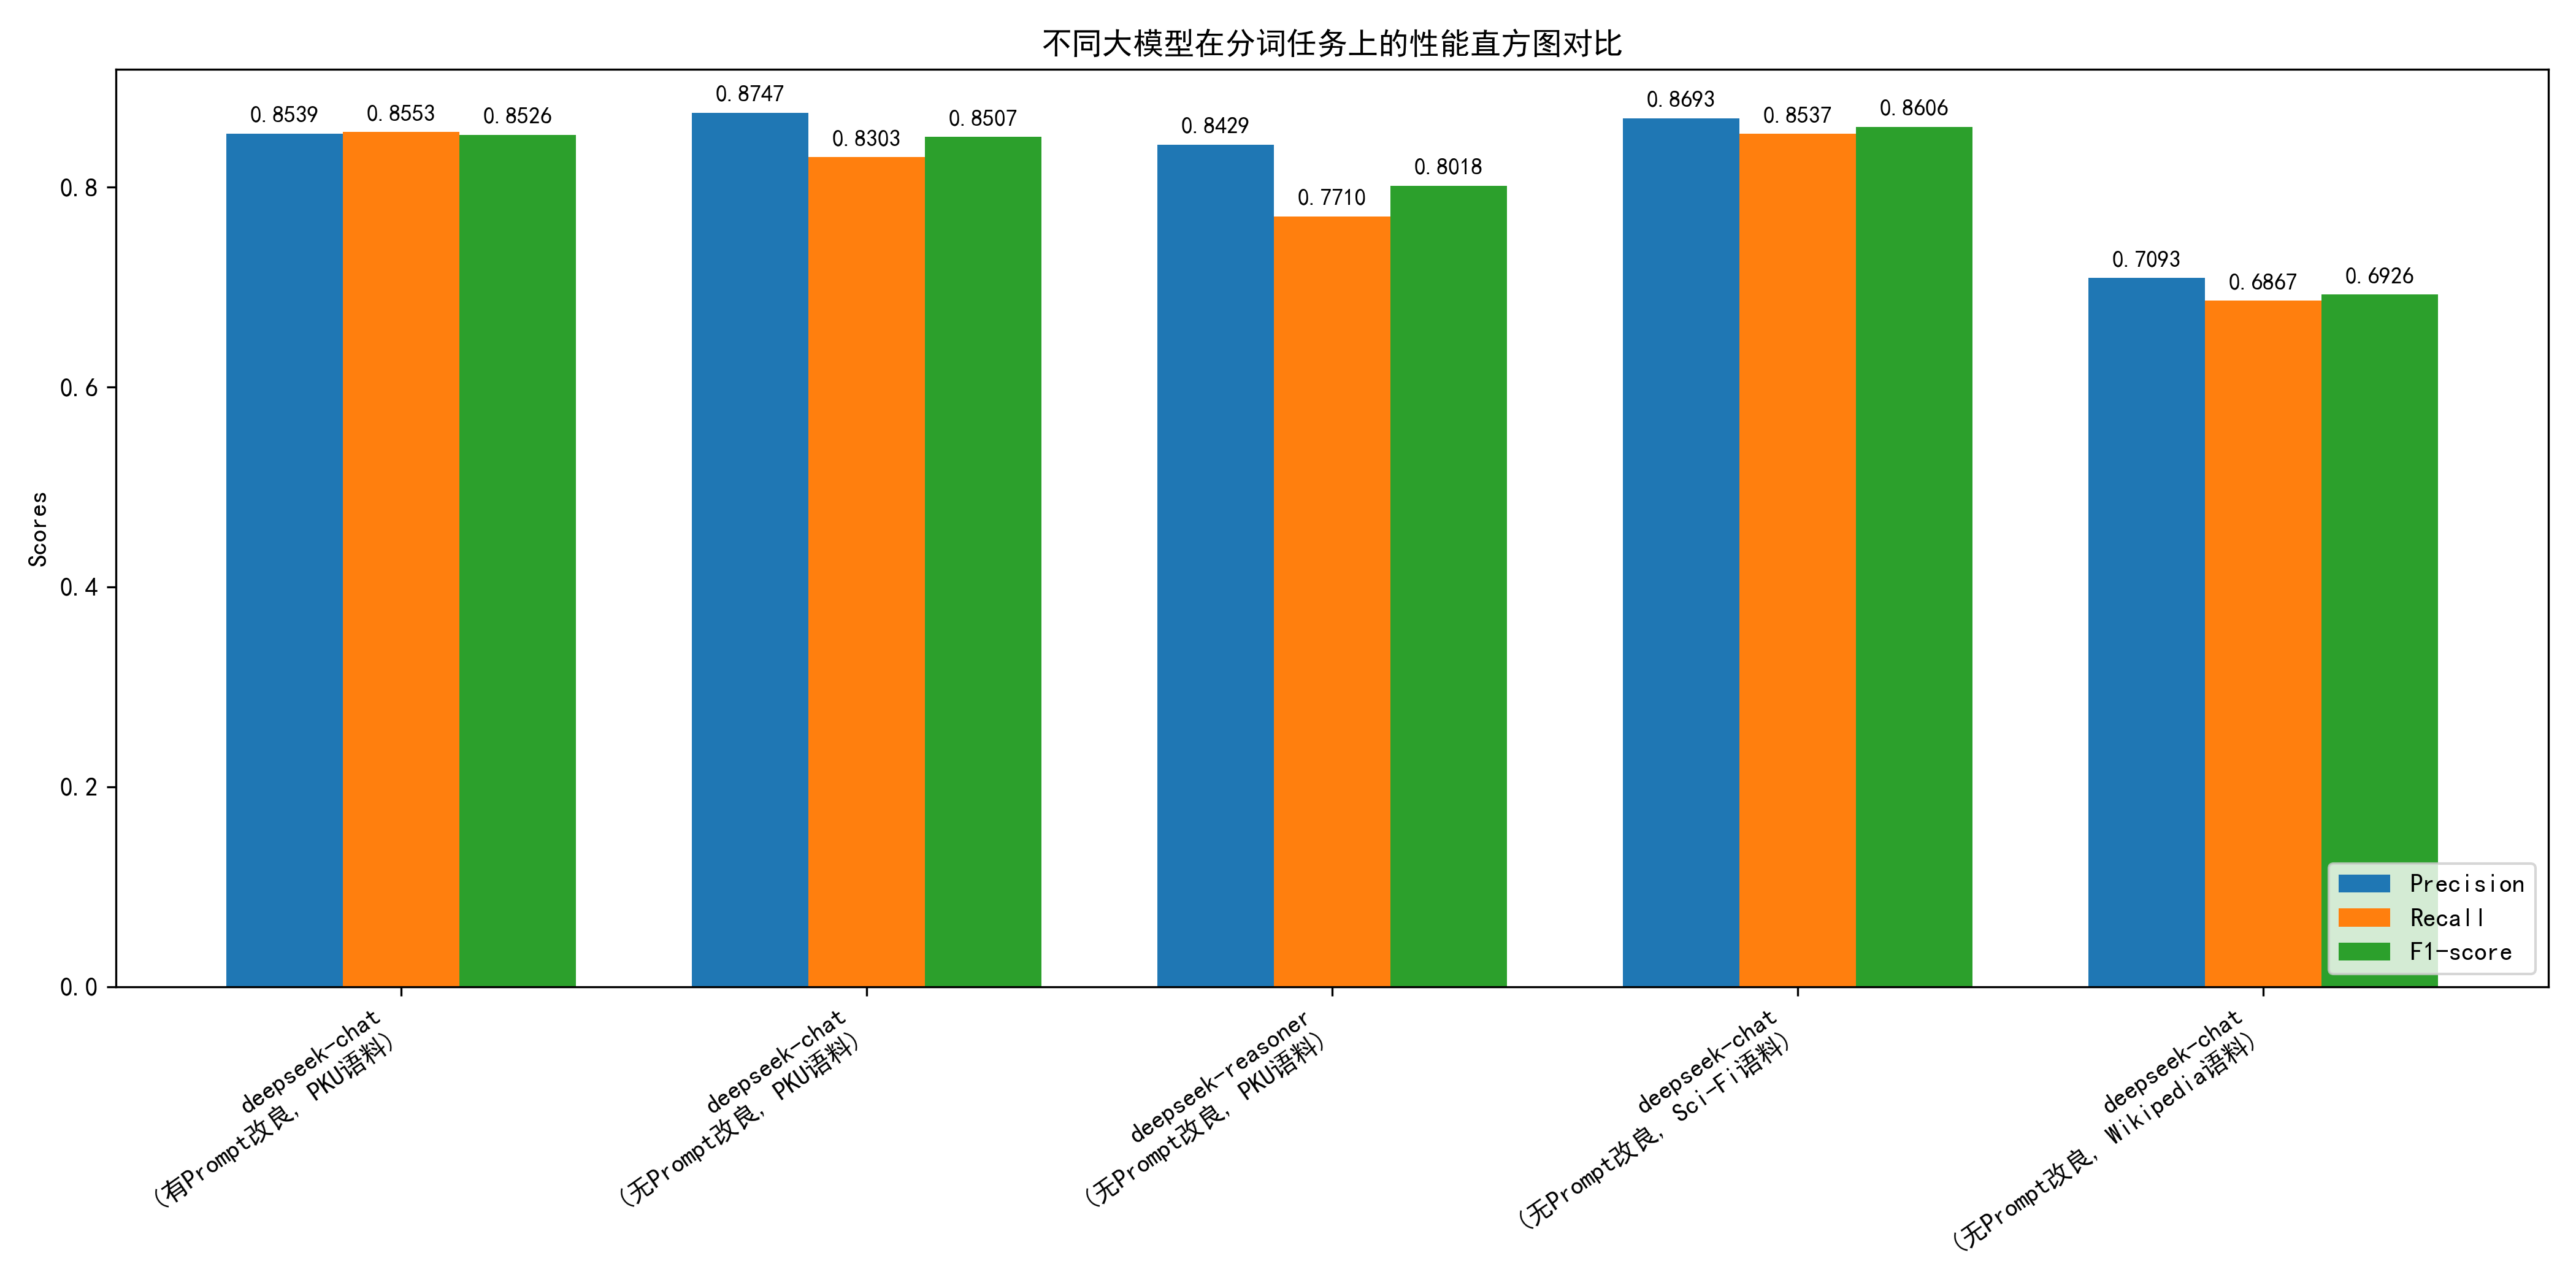
\includegraphics[width=1\textwidth]{fig/model_comparison.png}
    \caption{不同大模型在分词任务上的性能直方图对比}
\end{figure}
\end{document}